\documentclass[a4paper,12pt]{article}
\usepackage{amssymb}
\usepackage{amsmath}
\usepackage{hhline}
\usepackage{hyperref}
\usepackage{mathtools}
\usepackage{bm}
\usepackage[margin=2cm]{geometry}

\usepackage{amsthm}
\usepackage{mathptmx}


\usepackage{subcaption}

\usepackage{tabularx}
\usepackage{graphicx}
\usepackage{physics}
\usepackage{textcomp}


\graphicspath{ {./Images/} }


\newcommand{\code}[1]{\texttt{#1}}

\numberwithin{equation}{section}





\begin{document}
\title{\vspace{-3cm}\(1^{st}\) Challenge AN2DL}
\author{CorrectHorseBatteryStaple}
\date{}
\maketitle
In this report we intend to describe the steps we made during the \(1^{\text{st}}\) challenge of the AN2DL Course. It will be covered the structure of the dataset, the first steps we made, what we did right, what we did wrong and how we decided to finally tackle the problem.
\section*{Dataset}
The dataset we were given consists in \(3452\) photos of various species of plants. Inside the main folder there are \(8\) subdirectories. In every directory there are photos of the same plant. Aside from two directories, every species has about the same number of images. The first thing we noticed is the small size of the dataset. Having less then \(4000\)photos poses some limits on what we can do. Every image has a size of \(96 \times 96\) pixels, with \(3\) color channels. We opted for a 90\%/10\% split for the training and validation set.
\section*{Creating the Neural Network}
Since we were dealing with images, we opted for a Convolutional Neural Network (CNN), because we thought it was the best suited model for this kind of problem. We omitted talking about a model without data augmentation because at the first run it became clear that it would only lead to overfitting, a perfect accuracy with only a \(\approx 70\%\) validation accuracy, as the image below shows. 
\begin{figure}[h]
      \begin{subfigure}{0.5\textwidth}

      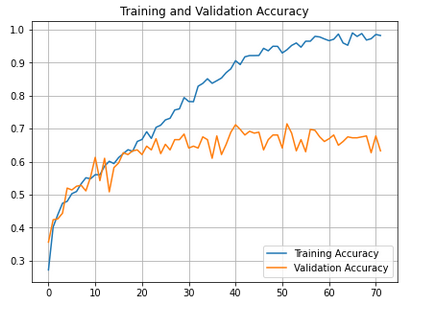
\includegraphics[scale=0.5]{model_noaug_acc.png}  
      \end{subfigure}
      \begin{subfigure}{0.4\textwidth}
            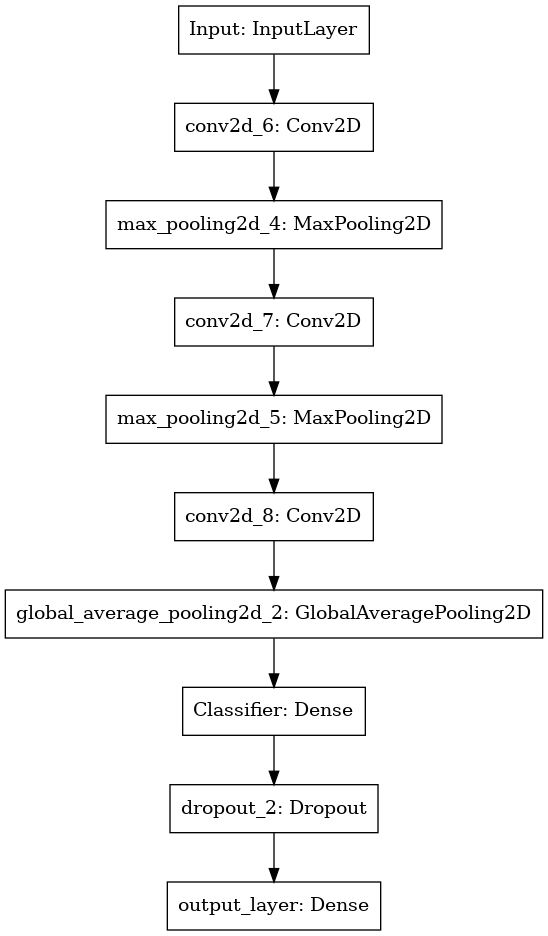
\includegraphics[scale=0.15]{model_noaug.png}
      \end{subfigure}
\end{figure}

Then, we tried to use data augmentation. Looking into Keras' documentation, we found that, inside the \code{layers} class, there were some layers specifically crafted to process images. In this way we avoided modifying the \code{model.py} file, which was a source of errors in our submissions. Using these preprocessing layers we created a \code{Sequential} model which contained our image augmentation. Here's an example of it, which we added as a layer inside every model we created after:
\begin{verbatim}
    
data_augmentation = tf.keras.Sequential([
      layers.RandomCrop(80, 80),
      layers.RandomFlip("horizontal_and_vertical"),
      layers.RandomRotation((-0.2, 0.2)),
      layers.Resizing(96,96, interpolation='bicubic'),
      layers.Rescaling(1./127.5, offset=-1)])
  
\end{verbatim}
We started by adding this simple preprocessing layer to our first net and we already saw some improvements. Afterwards, we decided that it would have been useful to implement a system that blocked the training in the moment it realizes that it's not imrpoving anymore. To solve this problem we used the callback method \code{EarlyStopping}. Using such method we avoided training a model for too may epochs if the model stopped improving its accuracy after a certain number of epochs. Then, trying with different learning rates and batch sizes, we quickly realized that we needed to update our architecture, so we started adding layers, making two convolutions before adding a pooling layer, but what really improved our CNN was the insertion of \code{SeparableConv2D} layers. Per Keras' documentation:
\begin{quote}
      Separable convolutions consist of first performing a depthwise spatial convolution (which acts on each input channel separately) followed by a pointwise convolution which mixes the resulting output channels.
\end{quote}
It's worth noting that also many of the pretrained architectures present inside the library make extensive use of this kind of layers. Our final CNN model was able to reach an accuracy of \(\approx 81\%\) on Codalab. All the notebooks with our code will be provided alongside this report.

After trying this approach we decided to follow the transfer learning method, in which we pass our dataset inside a Neural Network pretrained on bigger datasets. Inside the library there are quite a few options. We decided to try two pretrained nets: Xception and EfficientNetB7. 

The idea behind transfer learning and, subsequently, fine tuning is to give the dataset to a pretrained net, which has a precise set of weights, and then unfreeze the last layers such that part of the net can be trained on the dataset. In this way it is possible to reach outstanding accuracies from limited data. In our case, we tried a few different configurations, but the basic structure was composed by an input layer, followed by our data augmentation layer, then the pretrained model, a \code{Dense} layer and the output. Using Xception and fine tuning, we were able to reach an accuracy on the validation set of \(\approx 90\%\). 

Since Kaggle was providing us state of the art GPUs, we decided to take advantage and tried an even heavier net, EfficientNetB7. With over \(60\) millions parameters, it's one of the best performing net according to Keras' site. At some point we decided to set all the layers to trainable. We tried to add the method \code{ReduceLROnPlateau}, which gradually reduce the learning rate if the net isn't improving anymore. The EfficientNetB7 one was by far out best model and it performed well also on Codalab with a score of \(85\%\). We tried to change various parameters inside our fine tuned model, like the number of trainable layers, learning rate and all the things we could have changed (we tried different batch sizes, different augmentations, bigger or smaller classifier layers, etc...). But we couldn't find an idea to break the \(90\%\) ceiling, so we decided to use this result, which we still consider good. Looking forward to the next challenge to improve our work even more.
\section*{What we did right}
In this two section we try to understand how we worked, how many of the things we did were bringing us in the right direction and how many brought us to an halt. One of the main things that really helped us, was to look at the documentation available online (mainly Keras and Tensorflow's website). Looking into the documentation made more clear how the things we saw during the lesson, and the things our code was doing were really related. When we started we literally copy pasted the image classification lab code into a new notebook and adapted it for our dataset. Looking at the documentation helped us to find also alternative methods to approach problems. Creating a data augmentation layer enabled us to transfer a simple snippet of code to various notebooks without having to worry about compatibilty issues. 

Also, having a look at the architecture of the pretrained nets available prompted us to look more into the functioning of separable convolutions, since they were widely used. We were already aware that we couldn't reach the best results without transfer learning and fine tuning, but we still decided to spend some time crafting a net capable of reaching good results (\(\geq 80\%\)).
\section*{What we did wrong}
This section will be shorter than it should be, simply because if we knew other wrong things in our code we would have probably tried to solve it. But we were able to identify some of the errors we made that slowed down our progress. Since we are dealing with a programming task, it's obvious that every kind of error can happen, every typo, every mixed use of tab and spaces is a threat to our workflow, but this is not the focus of this section. Here we want to understand our conceptual errors. Our first major block was the complexity of the model. We started adding layers, putting bigger filters in our convolutions, and using a flattening layer. All these thing quickly added up, to the point in which even a basic CNN was able to have over \(40\) millions of trainable parameters. In this way we were creating overly complex nets, with no real gain in accuracy. It was starting to be time-consuming to train such a big network. The biggest drop in complexity came from getting rid of the flattening layer. Instead, we used a global pooling layer, which worked similarly to our max pooling layer, but gave us a tensor of the correct dimensions for the dense layer used as a classifier. That solution alone was able to stop the exponential growth of parameters of our CNN in a way that made impossible to train it using the hardware we had. 

When we moved to fine tuning, we found that more difficult than we imagined. When dealing with our own net, we had an idea of what was happening inside the model, with pretrained nets, we had the architecture, but some were made of over a hundred layers, so it was more difficult to debug problems. One of the major hiccup we found was unfreezing the layer and the forgetting to recompile the model. It may sound obvious, but, until we looked at the code we wrote in the lab about fine tuning, we didn't realize it. Also we aren't so sure why our best model was a net already available in Keras, but with no previous training, since we set all the model trainable. Maybe it's just a neural net really capable of doing image classification, but to us seems counterintuitive that leaving all the layers to train is the way to go if one is looking for a great accuracy. We tried unfreezing layers gradually and noticed this correlation between accuracy and number of trainable layers.
\end{document}
